\chapter{Penalised-Likelihood Reconstruction: Priors and Optimisation Algorithms}
\label{chapter:reconstruction}

Emission tomography reconstruction is an ill-posed inverse problem: the unknown activity must be inferred from noisy Poisson count data through a highly smoothing and poorly conditioned forward operator. While \acrfull{ml} approaches remain the clinical workhorse \cite{dempsterMaximumLikelihoodIncomplete1977, sheppMaximumLikelihoodReconstruction1982}, their practical success relies heavily on early stopping, which acts as an implicit regulariser but can introduce iteration-dependent bias and compromise quantification \cite{veklerovStoppingRuleMLE1987, wuConvergencePropertiesEM1983}. For quantitative, low-count, and multi-modality settings, precisely those that arise in modern \gls{pet}/\gls{spect} practice, explicit regularisation and fast, robust optimisation become essential.

This chapter reviews the modelling and algorithmic foundations that underpin the remainder of the thesis. We first formalise the Poisson statistical model and the penalised-likelihood reconstruction objective (often termed \acrfull{map}), highlighting where ill-conditioning and noise amplification enter the problem. We then present some regularisation strategies used in emission tomography: from classical quadratic smoothness priors and \acrfull{tv} \cite{rudinNonlinearTotalVariation1992}, through clinically deployed edge-preserving models such as the \acrfull{rdp} \cite{nuytsConcavePriorPenalizing2002}, to anatomically guided methods that use aligned structural images (e.g.\ Bowsher \cite{bowsherUtilizingMRIInformation2004}, \acrfull{pls} \cite{ehrhardtVectorValuedImageProcessing2014}, and kernelised representations \cite{wangPETImageReconstruction2015, hutchcroftAnatomicallyaidedPETReconstruction2016}. We then focus on synergistic regularisation, where multiple co-registered modalities are coupled during reconstruction, and motivate Jacobian-based vectorial priors such as \acrfull{jtv} and \acrfull{tnv} \cite{holtTotalNuclearVariation2014, rigieJointReconstructionMultichannel2015, knollJointMRPETReconstruction2017}, which will form the basis of the synergistic models developed later in the thesis.

Finally, we review optimisation algorithms suitable for large-scale \gls{map} reconstruction. After discussing EM-type updates and their subset-accelerated variants, we highlight why subset methods can exhibit limit-cycle behaviour and why convergent penalised algorithms typically require relaxation (e.g.\ \acrfull{bsrem} \cite{ahn_globally_2003}). We then introduce variance-reduced subset methods (e.g.\ \acrfull{saga} and \acrfull{svrg}) as a mechanism to retain low per-iteration cost while suppressing subset-induced stochasticity, and discuss the role of preconditioning, including ``prior-aware'' diagonal curvature approximations, in accelerating and stabilising convergence \cite{ehrhardtFastPETReconstruction2025a, twyman_investigation_2023}.


\section{The Inverse Problem in Emission Tomography}
\label{sec:recon_basics}

To discretely represent the spatial distribution of tracer concentration within a patient, the continuous activity distribution $f(r)$ is approximated using a basis expansion $f(r) \approx \sum_{j=1}^J x_j h_j(r)$. Typically, $\{h_j\}$ are chosen to be indicator functions on uniform cuboid voxels. In that case, it is customary to use a non-negative activity image vector $x = (x_1,\dots,x_J)^\top \in \mathbb{R}_+^{J}$.

The measured data consist of coincidence counts along lines of response (\gls{pet}) or projection bins (\gls{spect}). We denote the observed count in bin $i$ as $y_i$, and model it as a realisation of a Poisson counting process,
\begin{equation}
    y_i \sim \mathrm{Poisson}(Y_i),
    \qquad i=1,\dots,I,
\end{equation}
\noindent
where $Y_i=\mathbb E[y_i]$ is the (unknown) mean count, which we model as $Y_i \approx \bar y_i(x)$ with

\begin{align}
\bar y_i(x) = \sum_{j=1}^{J} a_{ij} x_j + b_i, \qquad i=1,\dots,I.
\end{align}
For notational simplicity, we will use the vector form
\begin{align}\label{eq:forward_model}
\bar y(x) = A x + b, \quad \quad \bar y_i(x) = (A x + b)_i,
\end{align}
where $A=[a_{ij}] \in \mathbb R_+^{I\times J}$ and $b\in\mathbb R_+^{I}$. Assuming independence of measurement bins, we obtain
\begin{equation}
p(y\mid x)
= \prod_{i=1}^I \frac{\bar{y}_i(x)^{y_i}\exp\!\left(-\bar{y}_i(x)\right)}{y_i!}.
\end{equation}
Taking logarithms yields the Poisson log-likelihood
\begin{equation}
\log p(y\mid x)
= \sum_{i=1}^I \left( y_i \log \bar{y}_i(x) - \bar{y}_i(x) - \log(y_i!) \right).
\end{equation}
Since the term $\sum_{i=1}^I \log(y_i!)$ does not depend on $x$, it can be dropped for optimisation purposes. Thus, maximising the likelihood w.r.t.~$x$ is equivalent to minimising
\begin{equation}
\mathcal{L}(x)
\coloneqq -\log p(y\mid x) + \mathrm{const}
= \sum_{i=1}^I \left( \bar{y}_i(x) - y_i \log \bar{y}_i(x) \right).
 \end{equation}

Unconstrained \gls{ml} solutions are dominated by noise due to the poor conditioning of $A$ and the Poisson noise inherent in $y$. While iterative \gls{em} methods such as \gls{mlem} and \gls{osem} \cite{dempsterMaximumLikelihoodIncomplete1977, sheppMaximumLikelihoodReconstruction1982} are the clinical standard, they rely on early stopping to act as an implicit regulariser. This yields clinically acceptable images but introduces solution-dependent bias that may not give reliable quantitative metrics \cite{veklerovStoppingRuleMLE1987}. In addition, finding the \gls{ml} solution for quantification can be prohibitively slow \cite{wuConvergencePropertiesEM1983}.

A robust alternative to early stopping is the Bayesian formulation. By Bayes' rule, we have
\begin{equation}
p(x\mid y) = \frac{p(y\mid x)\,p(x)}{p(y)},
\end{equation}
where $p(y\mid x)$ is the Poisson likelihood induced by the forward model, $p(x)$ encodes prior information about the unknown image, and the evidence
\begin{equation}
p(y) = \int p(y\mid x)\,p(x)\,\mathrm{d}x
\end{equation}
acts as a normalising constant independent of $x$.

A maximum a posteriori (\gls{map}) estimate is then defined as
\begin{equation}
\hat{x}_{\mathrm{MAP}} \in \arg\max_{x\in\mathcal{C}} \, p(x\mid y)
= \arg\max_{x\in\mathcal{C}} \, p(y\mid x)\,p(x),
\end{equation}
where $\mathcal{C}$ denotes a feasible set (typically enforcing non-negativity).
Taking negative logarithms, as above, gives an equivalent minimisation problem:
\begin{equation}
\hat{x}_{\mathrm{MAP}} \in \arg\min_{x\in\mathcal{C}}
\left\{-\log p(y\mid x) - \log p(x)\right\},
\end{equation}
since $-\log p(y)$ is constant with respect to $x$.

It is common to express the prior in Gibbs form,
\begin{equation}
p(x) \propto \exp\!\left(-\beta\,\mathcal{R}(x)\right),
\end{equation}
where $\mathcal{R}(x)$ is a regularisation functional and $\beta>0$ controls the strength of the prior. Substituting this into the \gls{map} objective yields the penalised-likelihood form
\begin{equation}
\hat{x}_{\mathrm{MAP}} \in \arg\min_{x\in\mathcal{C}}
\left\{\mathcal{L}(x) + \beta\,\mathcal{R}(x)\right\}.
\end{equation}


\section{Regularisation Strategies}

The choice of $\mathcal{R}(x)$ determines the texture and quantitative characteristics of the reconstructed image. Historically, this has evolved from simple smoothing constraints to sophisticated, anatomically guided models.

\subsection{Image-based Regularisation}
One of the simplest forms of regularisation is Tikhonov regularisation, which imposes an $\ell_2$-norm penalty on local voxel-wise differences. This yields the quadratic prior
\begin{equation}
    \mathcal{R}_{\mathrm{Quad}}(x)
    = \sum_{j=1}^J \sum_{k \in \mathcal{N}_j} w_{jk}\, (x_j - x_k)^2,
\end{equation}
where $\mathcal{N}_j$ denotes a local neighbourhood of voxel $j$ (e.g.\ 6, 18, or 26-connected in 3D) and $w_{jk}\ge 0$ are weights (often distance-based and symmetric). While strongly convex and computationally efficient, the quadratic penalty strongly discourages large local differences, which tends to oversmooth edges and suppress high-contrast structures \cite{gemanStochasticRelaxationGibbs1984}.

To better preserve edges, \gls{tv} \cite{rudinNonlinearTotalVariation1992} replaces the squared penalty with an $\ell_1$-type penalty on local differences. A neighbourhood-difference form that makes the connection to $\mathcal{R}_{\mathrm{Quad}}$ explicit is
\begin{equation}
    \mathcal{R}_{\mathrm{TV}}(x)
    = \sum_{j=1}^J \sum_{k \in \mathcal{N}_j} w_{jk}\, |x_j - x_k|.
\end{equation}
Relative to $\mathcal{R}_{\mathrm{Quad}}$, the linear growth of $|x_j-x_k|$ reduces the marginal cost of large voxel-wise jumps in intensity, thereby promoting piecewise-constant reconstructions with sharper edges.

In much of the imaging literature, \gls{tv} is instead written in terms of a discrete gradient operator. Defining $(D x)_j \in \mathbb{R}^d$ to collect finite differences at voxel $j$ along the $d$ coordinate directions, a common choice on a regular grid is
% Replace your Eq.~\eqref{eq:finite_difference} block with:
\begin{equation}
    \big((D x)_j\big)^{(\ell)}
    = \frac{x_{j+\delta_\ell} - x_{j}}{\Delta_{\ell}},
    \qquad \ell=1,\dots,d,
    \label{eq:finite_difference}
\end{equation}
where $\Delta_\ell$ denotes the Euclidean distance between voxels $j+\delta_\ell$ and $j$. The discrete TV functional is then
\begin{equation}
    \mathcal{R}_{\mathrm{TV}}(x)
    = \sum_{j=1}^J |(D x)_j|,
\end{equation}
with an isotropic alternative, more common in emission tomography \cite{jonssonTotalVariationRegularization1998, paninTotalVariationRegulated1999},
\begin{equation}\label{eq:tv}
        \mathcal{R}_{\mathrm{TV}}(x)
    = \sum_{j=1}^J \|(D x)_j\|_2.
\end{equation}

For optimisation, it is common to use a smooth approximation to avoid nondifferentiability at zero, for example
\begin{equation}
    \tilde{\mathcal{R}}_{\mathrm{TV}}(x)
    = \sum_{j=1}^J \sqrt{\|(D x)_j\|_2^2 + \epsilon^2},
    \qquad \epsilon>0.
\end{equation}

In clinical practice, adaptable edge-preserving priors are often preferred. The \gls{rdp} \cite{nuytsConcavePriorPenalizing2002}, the core component of the GE ``Q.Clear'' algorithm, modifies the penalty to depend on the absolute intensity sums, penalising relative differences, as opposed to absolute ones.
\begin{equation}
    \mathcal{R}_{\mathrm{RDP}}(x)
    = \frac{1}{2}\sum_{j=1}^J \sum_{k \in \mathcal{N}_j} w_{jk}
    \frac{(x_j-x_k)^2}{x_j+x_k + \gamma|x_j-x_k| + \epsilon},
    \label{eq:rdp}
\end{equation}
with $\gamma$ controlling the amount of edge preservation and $\epsilon\geq0$ the STIR RDP stabiliser. Positive $\epsilon$ regularises zero-valued voxel pairs; when $\epsilon=0$, STIR assigns the zero--zero contribution its limiting value of zero. Note that if $(x_j+x_k+\epsilon)\gg \gamma|x_j-x_k|$ then $\mathcal R_{\mathrm{RDP}}$ behaves like a relative quadratic prior,
whereas if $\gamma|x_j-x_k|\gg (x_j+x_k+\epsilon)$ it behaves like an anisotropic \gls{tv} penalty (up to a constant factor).

\subsection{Anatomically Guided Regularisation}
In low-count regimes, single-modality priors struggle to distinguish between noise and legitimate small structures. Anatomically guided reconstruction uses a high-resolution structural image $u$ (e.g., \gls{ct}) to modulate the regularisation of the emission image $x$.

Geometric Alignment methods assume that if an edge exists in the emission image, it should be supported by corresponding boundaries in a registered anatomical guidance image. The seminal Bowsher prior \cite{bowsherUtilizingMRIInformation2004} implements this idea by defining, for each voxel $j$, a data-adaptive and dynamic neighbourhood $\mathcal{B}_j(u)$ using the guidance image $u$. Concretely, from a fixed candidate neighbourhood $\mathcal{N}_j$, the Bowsher construction selects the $B$ voxels whose intensities in $u$ are most similar to $u_j$, i.e.\ those minimising a similarity metric such as
\begin{equation}
    d_{jk}(u) \coloneqq |u_j-u_k| \quad (k\in\mathcal{N}_j),
\end{equation}
and sets $\mathcal{B}_j(u)$ to be the indices of the $B$ smallest values of $d_{jk}(u)$. Regularisation is then applied only over this anatomically consistent subset, for example via a quadratic penalty
\begin{equation}
    \mathcal{R}_{\mathrm{Bow}}(x;u)
    = \sum_{j=1}^J \sum_{k\in \mathcal{B}_j(u)} w_{jk}\,(x_j-x_k)^2,
\end{equation}
(or an alternative edge-preserving potential). By restricting the penalty to neighbours that are locally homogeneous in $u$, the prior encourages smoothing within anatomical regions while reducing smoothing across anatomical edges, thereby allowing sharp boundaries to form in $x$ when they are supported by the guidance image.

An even more geometric framework is \gls{pls} \cite{ehrhardtVectorValuedImageProcessing2014}. These methods encourage structural consistency by encouraging the gradient vectors of the emission image and the guidance image to be aligned, i.e.\ $(D x)_j \parallel (D u)_j$. A common formulation (often termed \gls{pls}1) penalises the magnitude of the component of $(D x)_j$ orthogonal to $(D u)_j$, which is proportional to the sine of the enclosed angle $\theta_j$:
\begin{equation}
    R_{\mathrm{PLS1}}(x,u)
    = \sum_{j=1}^J \|(D x)_j\|_2\,\|(D u)_j\|_2\,|\sin\theta_j|.
\end{equation}
This term vanishes when $(D x)_j$ and $(D u)_j$ are parallel (or when either gradient is zero), and increases with the component of $(D x)_j$ orthogonal to $(D u)_j$. While numerically stable, \gls{pls}1 scales with $\|(D u)_j\|_2$ and therefore inherits the spatially varying gradient magnitude of the anatomical image, which can lead to over-weighting at strong anatomical edges and under-weighting in low-contrast regions.

To decouple the directional information from the anatomical gradient magnitude, \gls{dtv} \cite{ehrhardtPETReconstructionAnatomical2016} introduces a normalised direction field
\begin{equation}\label{eq:xi}
    \xi_j
    = \frac{(D u)_j}{\sqrt{\|(D u)_j\|_2^2 + \eta^2}},
\end{equation}
where $\eta>0$ is a small stabilisation parameter that  suppresses unreliable directions induced by noise or very fine-scale anatomical texture. Using $\xi_j$, one defines a local anisotropic projection operator
\begin{equation}\label{eq:directional_op}
    \Pi_j \coloneqq \mathbb{I} - \gamma_j\, \xi_j \xi_j^{\mathsf T},
\end{equation}
where $\mathbb{I}$ is the $d\times d$ (number of dimensions, $d$, squared) identity matrix and $\gamma_j\in[0,1]$ controls the strength of directional guidance. The resulting \gls{dtv} prior is
\begin{equation}\label{eq:dtv_defn}
    R_{\mathrm{dTV}}(x;u)
    = \sum_{j=1}^J \| \Pi_j (D x)_j \|_2,
\end{equation}
which penalises predominantly the gradient component orthogonal to the anatomical level-set direction, thereby encouraging edges in $x$ to align with edges in $u$. In regions where $u$ is locally flat (so $\xi_j \approx 0$), $\Pi_j \approx \mathbb{I}$ and \gls{dtv} reduces to standard isotropic \gls{tv}.

Regularisation strategies also exist outside the standard Bayesian (penalised-likelihood) framework. A prominent example is the \gls{kem}, in which prior information is encoded directly in the image representation rather than through an explicit penalty term. Following Wang and Qi \cite{wangPETImageReconstruction2015} and its anatomically-aided extension \cite{hutchcroftAnatomicallyaidedPETReconstruction2016}, the emission image is modelled as a linear combination of kernel-derived basis functions:
\begin{equation}
    x = K\alpha,
    \label{eq:kernel1}
\end{equation}
where $\alpha \in \mathbb{R}^J$ is a coefficient image and $K\in\mathbb{R}^{J\times J}$ is a (typically sparse) kernel matrix whose entries encode similarity between voxels based on features extracted from a guidance image \cite{hutchcroftAnatomicallyaidedPETReconstruction2016}. Each voxel $j$ is assigned a feature vector $f_j$ (commonly a patch of intensities in the high-resolution guidance image), and a radial Gaussian kernel is often used,
\begin{equation} \label{eq:gaussian_kernel}
    \kappa(f_j,f_k)=\
    \!\left(-\frac{\|f_j-f_k\|_2^2}{2\sigma^2}\right),
\end{equation}
with $\sigma$ controlling edge sensitivity. The kernel matrix is then defined entrywise by $K_{jk}=\kappa(f_j,f_k)$, with additional sparsification for tractability: for each voxel $j$, only a small set of the most similar neighbours (e.g.\ via a local $k$-nearest-neighbour search within a window) are allowed to contribute, yielding a sparse $K$. To preserve overall intensity scaling (counts), $K$ is typically row-normalised.

Substituting $x=K\alpha$ into the Poisson forward model gives a kernelised expectation for the data,
\begin{equation}
    \bar{y}(\alpha) = A(K\alpha) + b,
\end{equation}
so that reconstruction reduces to maximum-likelihood estimation of $\alpha$ under the same Poisson model, followed by $\hat{x}=K\hat{\alpha}$. Because the model remains linear in the unknown coefficients, an \gls{em}-type update can be derived with essentially the same structure as conventional MLEM/OSEM, but with $K$ embedded within the projector/backprojector operations. The resulting procedure is straightforward to implement in existing \gls{em} pipelines, and often improves the bias--variance trade-off at low counts by enforcing anatomically-informed, spatially adaptive smoothing in the image representation \cite{wangPETImageReconstruction2015,hutchcroftAnatomicallyaidedPETReconstruction2016}.

A known limitation of purely anatomy-derived kernels is \gls{pet}-unique feature suppression: structures present in the anatomical image but absent (or weak) in the emission image can be biased towards anatomically plausible but functionally incorrect solutions \cite{deiddaHybridPETMR2019}. To mitigate this, \gls{hkem} augments the kernel with synergistic information from the evolving \gls{pet} estimate itself, yielding an iteration-dependent kernel that combines anatomical and emission-driven similarity. In the \gls{hkem} formulation of Deidda \textit{et al.}, the hybrid kernel entry factorises as
\begin{equation}
    k^{(n)}_{fj} = k_m(v_f,v_j)\,k_p(z^{(n)}_f,z^{(n)}_j),
\end{equation}
where $v_j$ denotes the (fixed) anatomical feature vector at voxel $j$ and $z^{(n)}_j$ is a feature derived from the current \gls{pet} update (updated each iteration) \cite{deiddaHybridPETMR2019}. Both factors are commonly chosen as Gaussian similarities (Equation \ref{eq:gaussian_kernel} extended) modulated by spatial proximity,
\begin{align}
    k_m(v_j,v_k) &= \exp\!\left(-\frac{\|v_j-v_k\|_2^2}{2\sigma_a^2}\right)
                   \exp\!\left(-\frac{\|x_j-x_k\|_2^2}{2\sigma_{da}^2}\right),\\
    k_p(z^{(n)}_j,z^{(n)}_k) &= \exp\!\left(-\frac{\|z^{(n)}_j-z^{(n)}_k\|_2^2}{2\sigma_p^2}\right)
                   \exp\!\left(-\frac{\|x_j-x_k\|_2^2}{2\sigma_{df}^2}\right),
\end{align}
where $x_j$ denotes the voxel coordinates and the parameters $\sigma_a,\sigma_f,\sigma_{da},\sigma_{df}$ control the relative influence of anatomical similarity, functional-driven (emission) similarity, and spatial locality. The functional term helps address emission--guidance mismatch and reduces the tendency of anatomy-only kernels to suppress \gls{pet}-unique lesions by allowing the neighbourhood coupling to adapt to features emerging in the emission estimate. Empirically, Deidda \textit{et al.} report that this hybridisation can reduce negative bias under low-count conditions and improve lesion contrast while retaining the denoising benefits of kernelised reconstruction \cite{deiddaHybridPETMR2019}.

Kernel approaches extend naturally to multiple guidance sources by enlarging the feature vectors (e.g.\ concatenating features from \gls{ct} and/or additional functional channels \cite{wangPETImageReconstruction2015}) and defining the kernel on the resulting joint feature space. This provides a flexible mechanism for sequential or multi-modality guidance without introducing an explicit Bayesian penalty term. The kernel image model is applied to image-domain deconvolution in Chapter~\ref{chapter:deconvolution_pvc}.

\subsection{Synergistic Regularisation}\label{subsec:synergistic_recon}

If multiple modalities are available that depict the same underlying anatomy or functional distribution, it can be advantageous to reconstruct them synergistically, allowing information to be shared across modalities throughout the reconstruction process \cite{arridgeOverviewSynergisticReconstruction2021}. A prerequisite for such coupling is that the images are defined in a common spatial coordinate system. In practice, this requires geometric registration between modalities and resampling onto a common reconstruction grid, so that voxel index $n$ refers to the same physical location across all channels.

When the native modalities, indexed using $m$, are acquired on different grids or coordinate frames, we introduce spatial transforms $W_m$ (registration + resampling operators) and define the co-registered images on a shared grid, with $W_m: \mathbb{R}_+^{J_m} \rightarrow \mathbb{R}_+^N$:
\begin{equation}
    z_m \coloneqq W_m x_m \in \mathbb{R}_+^{N}, \qquad m=1,\dots,M,
\end{equation}
and collect them as the ordered modality tuple
\begin{equation}
    \bm{z} \coloneqq (z_1,\dots,z_M)
    \in (\mathbb{R}_+^N)^M
    \simeq \mathbb{R}_+^{N\times M},
\end{equation}
where the matrix-space identification stacks the modality images as columns.
Coupling priors are then naturally expressed in terms of $\bm{z}$, since neighbourhoods, gradients, and voxel-wise comparisons are only meaningful when images are spatially aligned.

In the Bayesian  setting, a generic multi-modality reconstruction is given by
\begin{equation}
    \hat{\bm{x}} \in \arg\min_{\bm{x}\in\mathcal{C}}
    \left\{
        \sum_{m=1}^M \mathcal{L}_m(x_m)
        + \beta\,\mathcal{R}(\bm{Wx})
    \right\},
\end{equation}
where $\bm{x}\coloneqq(x_1,\dots,x_M)$ and $\bm{W}\coloneqq\mathrm{diag}(W_1,\dots,W_M)$, and $\mathcal{R}(\bm{Wx})$ promotes cross-modality consistency (e.g.\ co-located edges or shared support) in the co-registered domain.

A practical way to exploit multiple modalities without solving a fully joint inverse problem is sequential reconstruction, in which one modality is first reconstructed, and the resulting image is then used as side-information to guide the reconstruction of another modality. In the Bayesian regime, this is
\begin{equation}
        \hat{x}_m \in \arg\min_{x_m\in\mathcal{C}}
\left\{\mathcal{L}_m(x_m) + \beta\,\mathcal{R}(x_m;W_{m\leftarrow(m-1)}x_{m-1})\right\},
\end{equation}
where $W_{m\leftarrow(m-1)}$ maps the image reconstructed in the previous stage, $x_{m-1}$, into the spatial grid of modality $m$.

Deidda et al.~have previously investigated a related method for \isotope[90]{Y} bremsstrahlung \gls{spect}--informed \gls{pet} reconstructions \cite{deiddaTripleModalityImage2023}. Bremsstrahlung \gls{spect} images are first reconstructed using \gls{hkem} with \gls{ct} and \gls{spect} image-update information to obtain an enhanced \gls{spect} estimate. This \gls{spect} image is then resampled to the \gls{pet} grid and used as functional guidance for \gls{pet} reconstruction.
\begin{equation}
    \hat{\alpha}_m \in \arg\min_{\alpha_m\in\mathcal{C}}
    \left\{
        \mathcal{L}_m\!\left(W_{m\leftarrow(m-1)}\,K_m\alpha_m\right)
    \right\}.
\end{equation}
The paper reports that this sequential design is particularly beneficial for low-count \gls{y90} \gls{pet}: \gls{spect} provides complementary denoising/uptake support within \gls{pet}--\gls{spect}-consistent regions, while \glsentryshort{ct} contributes primarily through resolution/edge information injected at the \gls{spect} stage, and the \gls{pet} image-update features reduce suppression of \gls{pet}-unique structures and mitigate inter-modality mismatch.

Sequential guidance is limited by one-way dependency: errors in $u$ may propagate directly to $x$ and the shared information may not be fully utilised. Truly synergistic reconstruction estimates both images simultaneously, allowing information to flow bi-directionally. Perhaps the most obvious way to extend single modality regularisation to achieve a synergistic regulariser is \gls{jtv} \cite{blomgrenColorTVTotal1998}, a simple extension of TV which sums gradient magnitudes:
\begin{equation}
    \mathcal{R}_{\mathrm{JTV}}(\bm{z}) = \sum_{n=1}^N \sqrt{ \|D z_{1,n}\|^2 + \|D z_{2,n}\|^2 + \dots +\|D z_{M,n}\|^2 }.
\end{equation}
This encourages joint sparsity, encouraging co-located edges. A convenient way to formalise multi-modality edge co-localisation is to view the set of images as a vector-valued field.  For each voxel $n$, the voxel-wise Jacobian is defined by stacking image gradients (Equation \ref{eq:finite_difference}) in columns:
\begin{equation}\label{eq:jacobian}
\mathcal{G}_n(\bm{z})
\;\coloneqq\;
\begin{bmatrix}
D z_{1,n} & D z_{2,n} & \cdots & D z_{M,n}
\end{bmatrix}
\;\in\; \mathbb{R}^{d\times M}.
\end{equation}
When viewed in this way, \gls{jtv} can be redefined as a Schatten $2$-norm (also known as a Frobenius norm) applied to this jacobian \cite{holtTotalNuclearVariation2014},
\begin{equation}\label{eq:jtv}
    \mathcal{R}_{\mathrm{JTV}}(\bm{z}) = \sum_{n=1}^N  \|\mathcal{G}_n(\bm{z})\|_F
\end{equation}
where the Schatten $p$-norm is defined as
\begin{equation}\label{eq:schatten}
    \|Y\|_{Sp} \coloneqq \left(\sum_{r=1}^{R}\sigma_r(Y)^p\right)^{1/p}
\end{equation}
for singular values $\sigma_\ell(Y)$ of a rank-$R$ matrix $Y$. Note that $R=\min\{d,M\}$. The Schatten $1$-norm, also known as the nuclear norm is the sum of singular values
\begin{equation}
    \|Y\|_* = \sum_{r=1}^{R}\sigma_r(Y).
\end{equation}
The nuclear norm is the convex envelope of the Rank function. Applied to the voxel-wise jacobians, it promotes singular value sparsity and has the effect of either driving functionally misaligned gradients to zero or parallel/anti-parallel, promoting edge-alignment. Applying this nuclear norm to the voxel-wise jacobians is known as \gls{tnv} \cite{holtTotalNuclearVariation2014, rigieJointReconstructionMultichannel2015}.
\begin{equation}\label{eq:tnv}
    \mathcal{R}_{\mathrm{TNV}}(\bm{z}) = \sum_{n=1}^N  \|\mathcal{G}_n(\bm{z})\|_*
\end{equation}
It has been applied to synergistic \gls{pet}/MR reconstruction through its extended variant, total generalised nuclear variation \cite{knollJointMRPETReconstruction2017}.

The benefits of using the nuclear norm over the Frobenius norm can be visualised in Figure~\ref{fig:norm_visualisation}, where the nuclear norm exhibits sharp grooves along the coordinate axes that encourage one singular value to vanish (promoting low-rank structure), whereas the Frobenius norm is smooth and tends to shrink singular values jointly without explicitly favouring rank reduction.

\begin{figure}[hbtp]
    \centering
    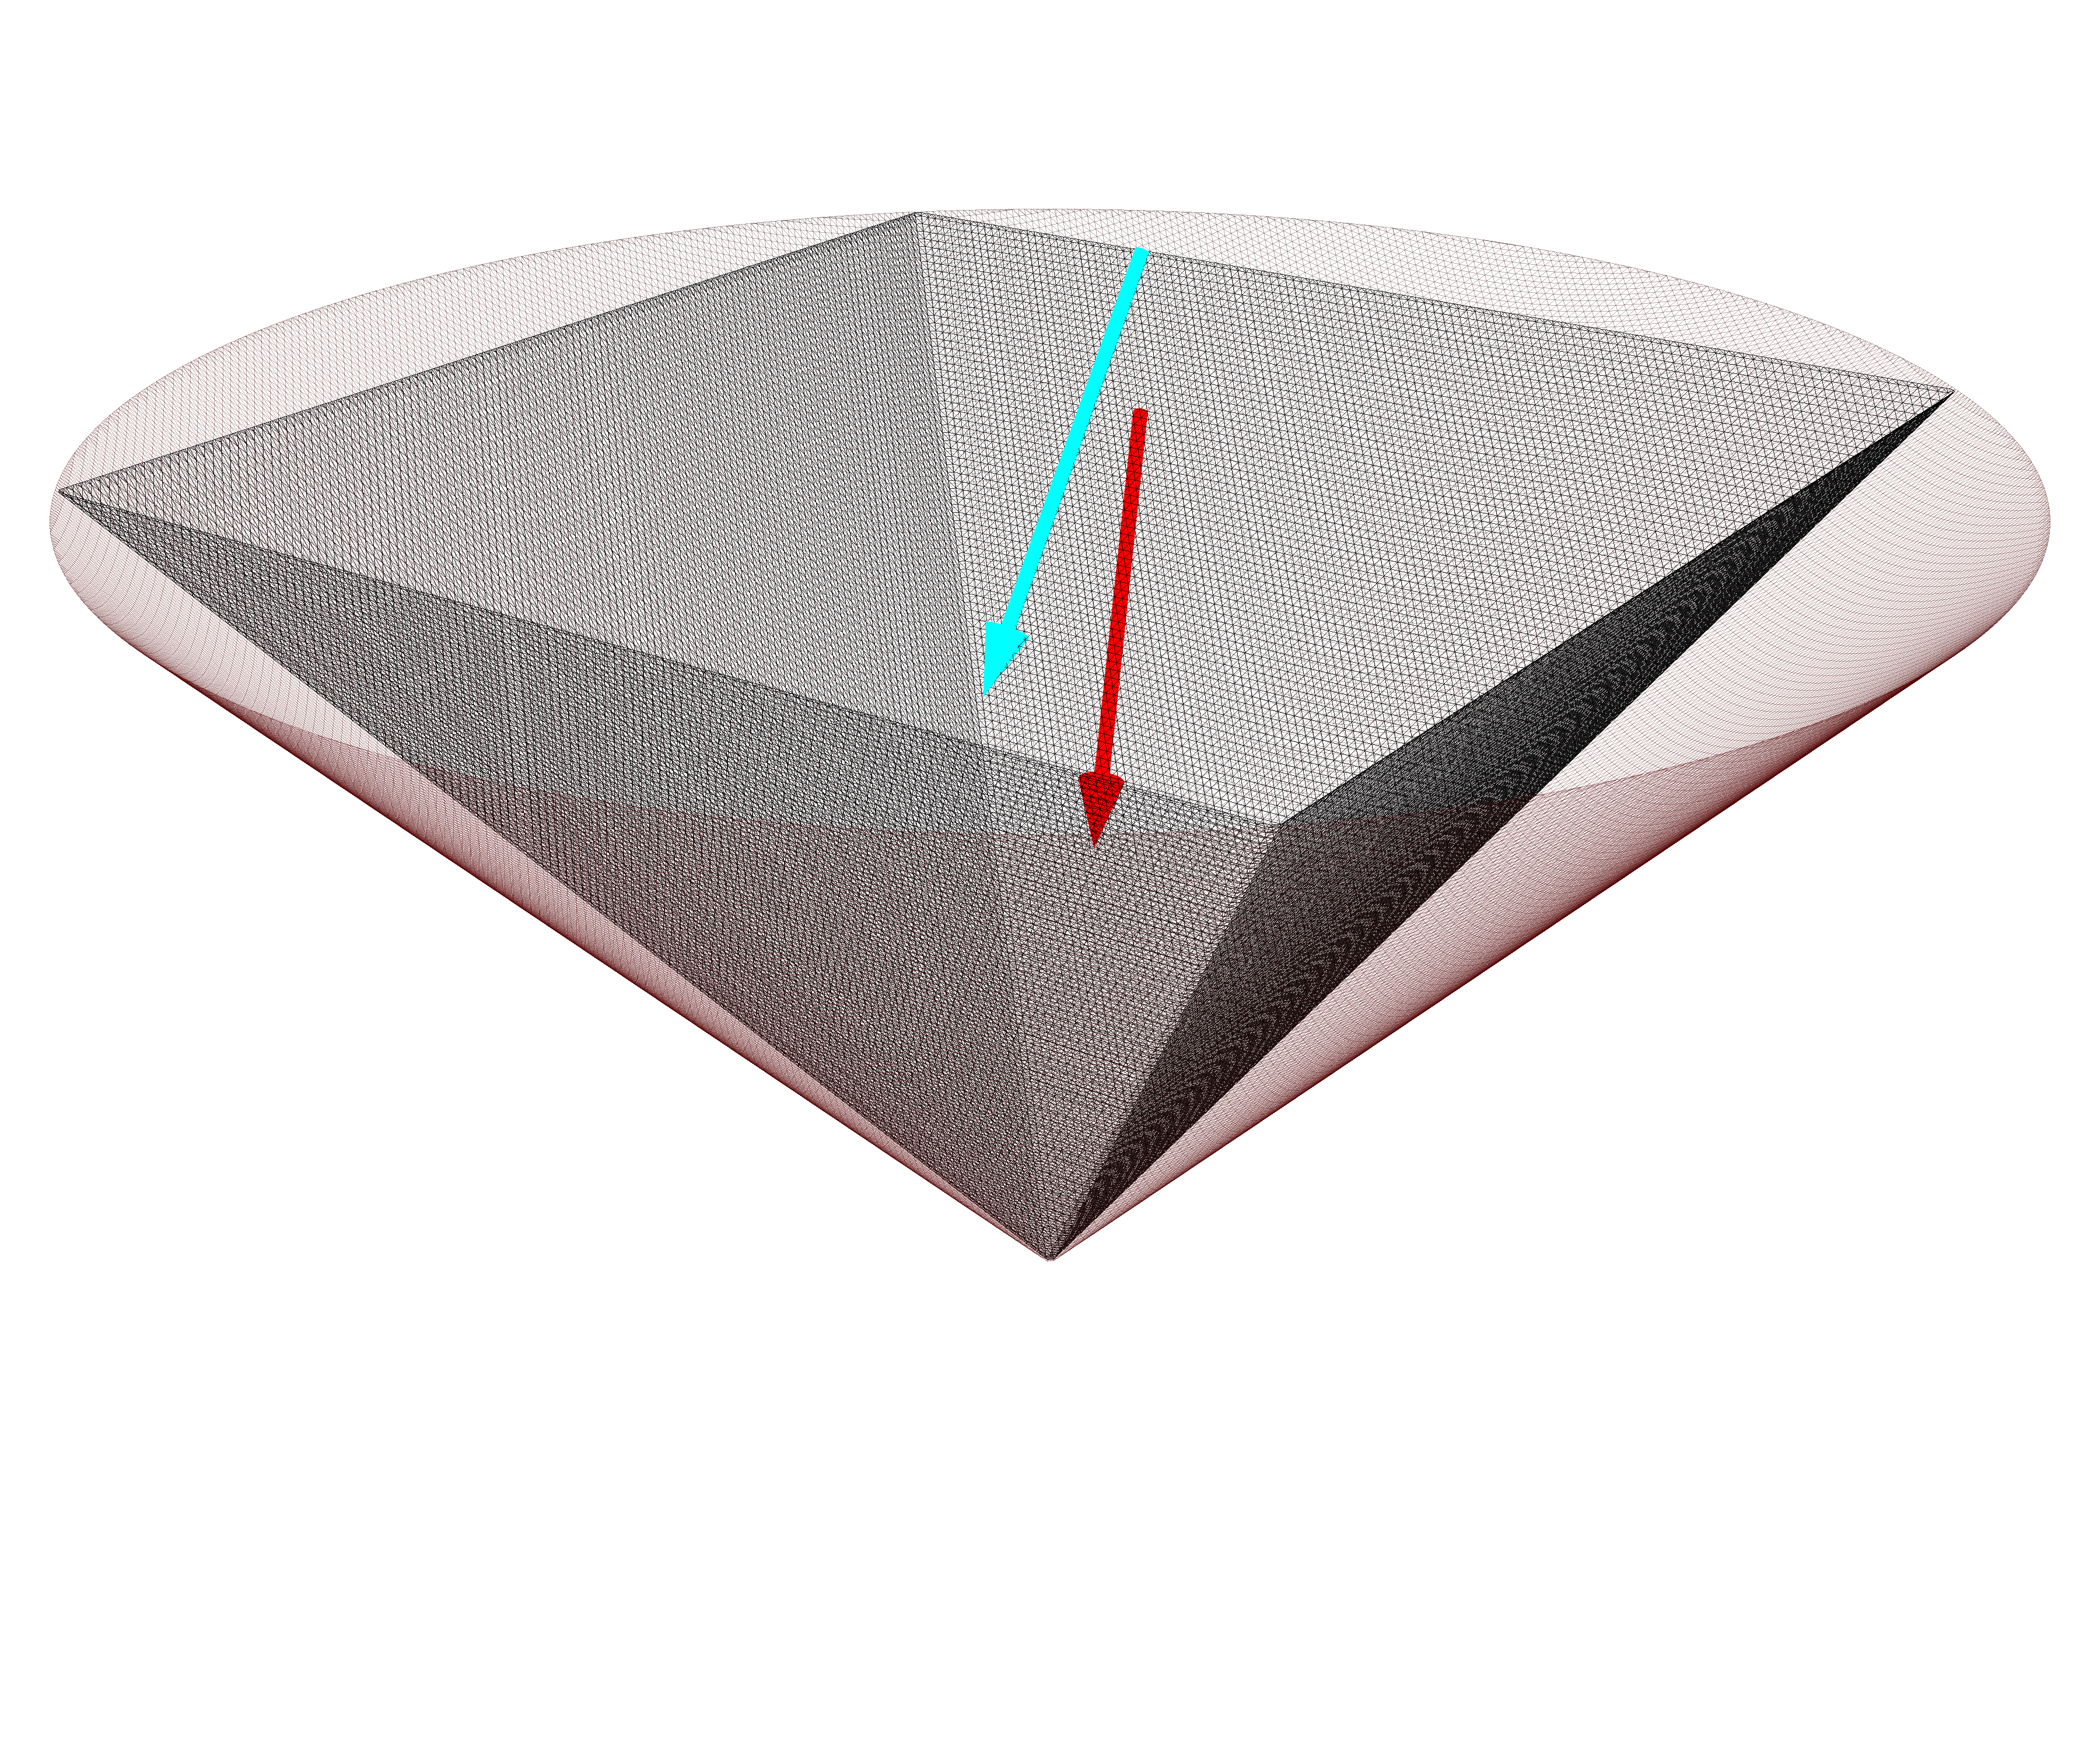
\includegraphics[trim={1cm 20cm 1cm 0},clip, width=0.85\linewidth]{figures/Chapter4/norm_visualisation.png}
    \caption{Visualisation of the Frobenius and nuclear norms (vertical axis) of a matrix $X$ as functions of its (two) singular values (horizontal axis). The Frobenius norm is $\|X\|_F=\sqrt{\sigma_1(X)^2+\sigma_2(X)^2}$ (red mesh), whereas the nuclear norm is $\|X\|_* = |\sigma_1(X)|+|\sigma_2(X)|$ (black mesh). For visualisation purposes we extend the singular-value axes to negative values. The nuclear norm exhibits sharp grooves along the coordinate axes, encouraging one singular value to vanish (i.e.\ promoting low-rank structure), while the Frobenius norm is smooth and does not preferentially drive a singular value exactly to zero. This behaviour can also be understood via subgradients: the nuclear-norm subgradient (cyan) points towards rank-1 grooves, preferentially shrinking the smaller singular value, whereas the Frobenius-norm subgradient (red) points towards the origin, shrinking both singular values equally.}
    \label{fig:norm_visualisation}
\end{figure}

Total Nuclear variation will form the basis for the synergistic prior demonstrated later on in this thesis.

\section{Optimisation Algorithms}\label{sec:optimisation}

\gls{mlem} has the multiplicative update equation for iteration $k$:
\begin{equation}
    x^{(k+1)}
    =
    \left( x^{(k)} \oslash A^{\mathsf T} \mathbf{1}_I \right) \odot
        A^{\mathsf T}\!\left(\, y \oslash \bar{y}\right)
,
\end{equation}
where $\odot$ and $\oslash$ denote elementwise multiplication and division, respectively, $\mathbf{1}_I\in\mathbb{R}^{I}$ is an all-ones vector and $k$ denotes the iteration number. For notational simplicity, we drop the explicit elementwise operators so that all divisions are understood componentwise. Then
\begin{equation}
x^{(k+1)}
=
\operatorname{diag}\!\left(\frac{x^{(k)}}{A^{\mathsf T}\mathbf{1}_I}\right)\,
A^{\mathsf T}\!\left(\frac{y}{\bar{y}}\right).
\end{equation}

This can be rearranged to form the additive update equation
\begin{align}
    x^{(k+1)}
    & = x^{(k)} +
    \operatorname{diag}\!\left(\frac{x^{(k)}}{A^{\mathsf T}\mathbf{1}_I}\right)
        A^{\mathsf T}\!\left(\frac{y}{\bar{y}\!\left(x^{(k)}\right)} -\mathbf{1}_I \right) \nonumber \\
     & = x^{(k)} -
    \operatorname{diag}\!\left(\frac{x^{(k)}}{A^{\mathsf T}\mathbf{1}_I}\right)
        \nabla_x \mathcal{L}(x^{(k)}).
\end{align}
where $\mathbf{1}_J\in\mathbb{R}^{J}$ is an all-ones vector. This form highlights that the \glsentryshort{mlem} update can be interpreted as a preconditioned gradient descent algorithm with preconditioner $\mathcal{P}_{\mathrm{EM}}^{(k)}=\operatorname{diag}\!\left(\frac{x^{(k)}}{A^{\mathsf T}\mathbf{1}_I}\right)$, i.e.
\begin{align}
    x^{(k+1)} = x^{(k)} - \varsigma \mathcal{P}_{\mathrm{EM}}^{(k)} \nabla_x \mathcal{L}(x^{(k)}),
\end{align}
with a step size $\varsigma=1$.

A preconditioner aims to recondition the reconstruction space so that gradient steps are appropriately scaled across voxels, improving numerical conditioning and convergence. Intuitively, we seek larger steps in poorly sensitive directions and smaller steps in highly sensitive directions, thereby approximating curvature information.

Subsets are commonly used to accelerate early convergence by partitioning the data into $S$ subsets and updating the image using only the contribution from a single subset (or a small batch of subsets) at each iteration. Writing the negative log-likelihood as a sum of subset terms,
\begin{equation}
    \mathcal{L}(x)=\sum_{s=1}^S \mathcal{L}_s(x),
\end{equation}
a generic subset scaled-gradient update takes the form
\begin{equation}
    x^{(k+1)}
    =
    x^{(k)} - \varsigma\,\mathcal{P}^{(k)}\,\nabla_x \mathcal{L}_{s}\!\left(x^{(k)}\right).
\end{equation}
If multiple subsets are used per iteration, $\nabla_x \mathcal{L}_{s}$ can be replaced by an average over the chosen subset indices. The most common algorithm found in clinical systems is the \gls{osem} algorithm. For subset $s$ at iteration $k$, a standard \glsentryshort{osem} update can be written as
\begin{equation}
x^{(k+1)}
=
\operatorname{diag}\!\left(\frac{x^{(k)}}{A_s^{\mathsf T}\mathbf{1}_I}\right)\,
A_s^{\mathsf T}\!\left(\frac{y_s}{\bar{y}_s\!\left(x^{(k)}\right)}\right),
\end{equation}
where $A_s$ denotes the system matrix and data restricted to subset $s$. \gls{osem} cycles through subsets incrementally.

\glsentryshort{osem} typically shows a marked improvement in early-stage convergence by providing a cheaper approximation of the full-data \glsentryshort{em} update. However, because the subset gradient is only an approximation to the full gradient, \glsentryshort{osem} is not, in general, a convergent algorithm for the maximum-likelihood problem: as the iterates approach a solution, incremental sub-gradient updates can lead to cyclical behaviour. An example illustrating this is shown in  Figure~\ref{fig:osem_limit_cycle}.

\begin{figure}[htbp]
    \centering
    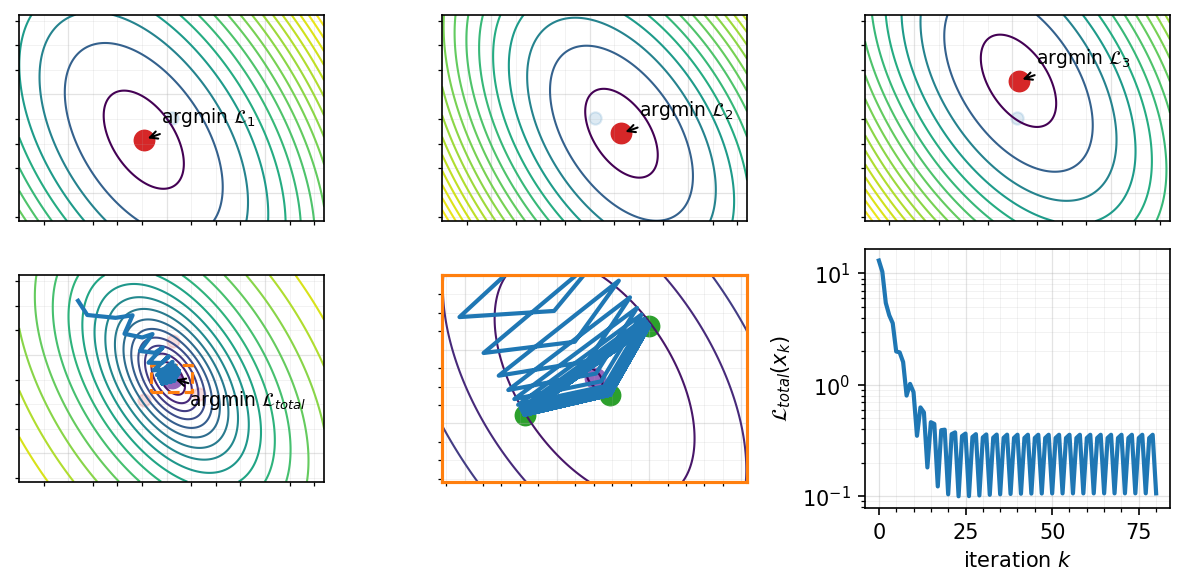
\includegraphics[width=\linewidth]{figures/Chapter2/osem_limit_cycle.png}
    \caption{Demonstration of limit cycle behaviour with an ordered subset gradient descent algorithm. Top row: 3 different simple binomial sub-functions representing subset likelihoods. Bottom row: left, full function with sub-gradient steps; centre, zoomed version of the full function demonstrating limit cycle behaviour (green dots show approximate points of limit cycle); right, likelihood value per iteration, demonstrating thre limit cycle.}
    \label{fig:osem_limit_cycle}
\end{figure}

We seek a fast and convergent algorithm for \gls{map} reconstruction. A widely used approach is the (modified) \gls{bsrem} framework \cite{depierroFastEMlikeMethods2001, ahn_globally_2003}, which combines \glsentryshort{em}-type preconditioning and subset acceleration with a relaxation (diminishing step-size) to recover convergence while incorporating an explicit penalty. In a scaled-gradient form, a generic \glsentryshort{bsrem}-type update can be written as
\begin{equation}
    x^{(k+1)}
    =
    x^{(k)} - \varsigma_k\,\mathcal{P}_{\mathrm{EM}}^{(k)}
    \left(
        \nabla_x \mathcal{L}_s(x^{(k)})
        + \frac{\beta}{S}\,\nabla_x \mathcal{R}(x^{(k)})
    \right),
\end{equation}
where $\varsigma_k>0$ is an iteration dependent step size. Convergence is promoted by choosing $\{\varsigma_k\}$ to diminish appropriately (e.g.\ $\varsigma_k\rightarrow 0$ with $\sum_k \varsigma_k=\infty$), which suppresses the subset-induced limit-cycle behaviour while retaining rapid early progress (see Figure~\ref{fig:relaxed_limit_cycle}).

\begin{figure}[htbp]
    \centering
    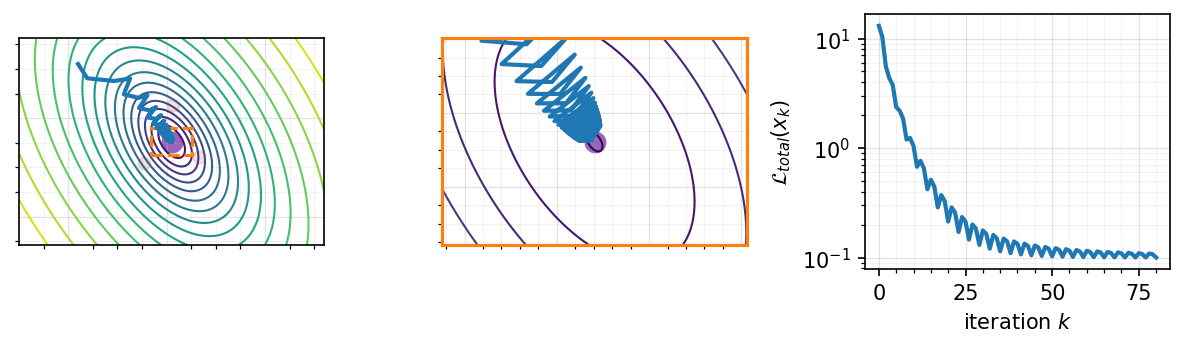
\includegraphics[width=\linewidth]{figures/Chapter2/relaxed_limit_cycle.png}
    \caption{Demonstration of reduction in limit cycle behaviour with step size relaxation $\varsigma_k=\varsigma_0/(1+0.05k)$. Left, full function with sub-gradient steps; centre, zoomed version of the full function demonstrating relaxed limit cycle behaviour; right, likelihood value per iteration, demonstrating relaxed limit cycle precession. }
    \label{fig:relaxed_limit_cycle}
\end{figure}

Variance-reduced subset methods have become increasingly popular in the \gls{pet} reconstruction literature because they retain the low per-iteration cost of subset updates while substantially reducing the limit cycling observed in \gls{osem}. The key idea is to replace the raw subset gradient, which is a high-variance estimator of the full gradient, with a variance-reduced estimator that is (approximately) unbiased and whose variance decreases as the iterates approach a solution \cite{ehrhardtFastPETReconstruction2025a,twyman_investigation_2023}.

A stochastic subset gradient step uses $g_{s_k}(x^{(k)})$ in place of $\nabla \mathcal{L}(x^{(k)})=\sum_s g_s(x^{(k)})$, i.e.
\begin{equation}
    x^{(k+1)}
    = x^{(k)} - \varsigma_k\,\mathcal{P}^{(k)}
    g_{s_k}(x^{(k)}),
\end{equation}
which is cheap but noisy. Variance reduction augments this step by incorporating additional information (stored gradients or periodic full-gradient computations) to form a corrected estimator $\tilde g_k$ with reduced variance. Two widely used examples are \gls{saga} and \gls{svrg}:

\gls{saga} \cite{defazio_saga_2014} maintains a table of the most recently computed subset gradients $\{g_s(\cdot)\}_{s=1}^S$ and updates using
\begin{equation}
    \tilde g_k
    \;=\;
    g_{s_k}(x^{(k)}) - g_{s_k}(\tilde x_{s_k}) + \frac{1}{S}\sum_{s=1}^{S} g_s(\tilde x_s),
\end{equation}
where $\tilde x_s$ denotes the iterate at which the stored gradient for subset $s$ was last evaluated.

\gls{svrg} \cite{johnsonAcceleratingStochasticGradient2013} periodically computes a reference full gradient at a snapshot $\tilde x$ and then performs inner iterations using
\begin{equation}
    \tilde g_k
    \;=\;
    g_{s_k}(x^{(k)}) - g_{s_k}(\tilde x) + \nabla_x \mathcal{L}(\tilde x).
\end{equation}
In both cases, $\tilde g_k$ is designed so that $\mathbb{E}[\tilde g_k]\approx 1/S \;\nabla_x \mathcal{L}(x^{(k)})$ while its variance decreases as $x^{(k)}$ approaches a stationary point, thereby mitigating the oscillatory behaviour seen in OSEM and improving stability at high iteration counts (see Figure~\ref{fig:svrg_limit_cycle}).

\begin{figure}[htbp]
    \centering
    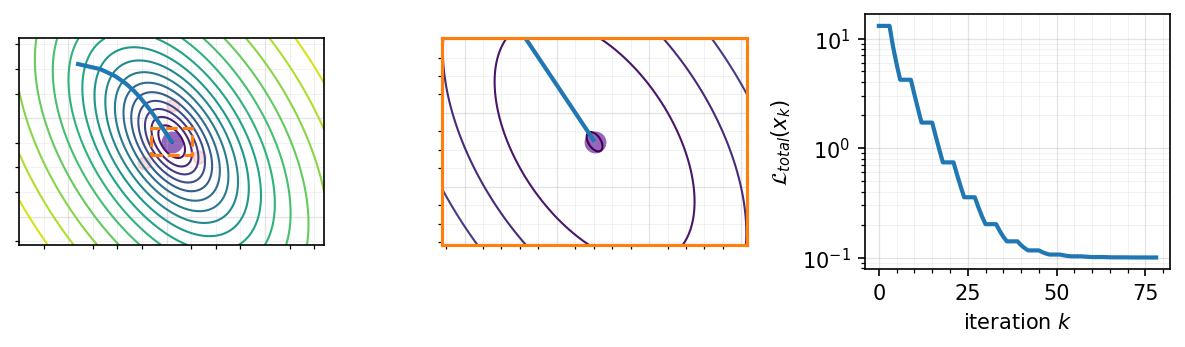
\includegraphics[width=\linewidth]{figures/Chapter2/svrg_limit_cycle.png}
    \caption{Demonstration of removal of limit cycle behaviour with an \gls{svrg}-type (Ordered VRG) algorithm. Left, full function with sub-gradient steps; centre, zoomed version of the full function demonstrating removal of limit cycle behaviour; right, likelihood value per iteration, demonstrating removal of limit cycle precession }
    \label{fig:svrg_limit_cycle}
\end{figure}

A variance-reduced, prior-regularised update can then be written compactly as
\begin{equation}
    x^{(k+1)}
    = x^{(k)} - \varsigma\,\mathcal{P}^{(k)}
    \Big(\tilde g_k + \beta \nabla_x\mathcal{R}(x^{(k)})\Big).
\end{equation}
Recent work indicates that incorporating the effect of the prior into $\mathcal{P}^{(k)}$ (``prior-aware preconditioning'') can substantially accelerate convergence. Ehrhardt \textit{et al.} \cite{ehrhardtFastPETReconstruction2025a} showed substantially improved convergence rates with \gls{rdp}-regularised \gls{pet} reconstruction when using harmonic averaging of the \gls{em}-type preconditioner and a scaled diagonal estimate of the inverse Hessian of the prior. Using only the diagonal elements of the \gls{rdp} Hessian
\begin{equation}
    [\mathcal{H}_{\mathrm{RDP}}(x)]_{jj}
    = \sum_{k \in \mathcal{N}_j}
    \frac{2w_{jk}(2x_k+\epsilon)^2}
    {(x_j + x_k + \gamma |x_j - x_k|+\epsilon)^3},
\end{equation}
they constructed a preconditioner as
\begin{equation}
    \mathcal{P}^{(k)} = \operatorname{diag}\left( \frac{x^{(k)}+\delta}{A^\top \mathbf{1} + \alpha \;\operatorname{diag}\!\left(\beta \mathcal{H}_{\mathrm{RDP}}\left(x^{(k)}\right)\right)\left(x^{(k)}+\delta\right)}\right)
\end{equation}
with scalar $\alpha$ tuned to correct for the loss of off-diagonal information. 
\begin{comment}
Although this is not emphasised explicitly in \cite{ehrhardtFastPETReconstruction2025a}, the harmonic averaging viewpoint can also be interpreted as a majorisation-preserving way to combine curvature information from the likelihood and the prior. In particular, the voxel-wise harmonic blend can be rearranged as
\begin{equation}
\left(\frac{1}{a}+\frac{1}{b}\right)^{-1},
\end{equation}
so that combining two diagonal scalings $a$ and $b$ harmonically is equivalent to inverting the sum of the corresponding inverse-scalings (i.e.\ two diagonal Hessian surrogates). Consequently, when these inverse-scalings are chosen as upper-bounding approximations of the respective Hessians, their sum remains a valid upper bound, and the resulting harmonic combination inherits this majorising property while still incorporating both data-fidelity and prior-induced curvature.
\end{comment}

Preconditioning and stochastic variance reduction for synergistic \gls{map} reconstruction has not been well investigated in the literature so far and will form a part of this thesis.

A widely used alternative to \gls{em}-type and subset-gradient schemes is the limited-memory BFGS algorithm with bound constraints (L-BFGS-B) \cite{broydenConvergenceClassDoublerank1970, fletcherNewApproachVariable1970, goldfarbFamilyVariablemetricMethods1970, shannoConditioningQuasiNewtonMethods1970, liuLimitedMemoryBFGS1989, byrd_limited_1995, zhuAlgorithm778LBFGSB1997}, a quasi-Newton method that iteratively builds a low-rank approximation to the inverse Hessian from successive iterate and gradient differences. The “limited-memory” construction stores only a small number of correction pairs, making it viable for high-dimensional images, while the “B” variant enforces simple bounds (e.g.\ non-negativity) via an active-set strategy and projected search directions. 

In practice, L-BFGS-B can exhibit rapid local convergence on smooth penalised objectives, but each iteration requires one or more full objective and gradient evaluations (coupled with a line search), which is computationally burdensome in large-scale emission tomography when the likelihood is evaluated over all subsets. For this reason it is not used in the main reconstruction experiments in this thesis. Nevertheless, it provides a useful reference optimiser and is employed later for a small demonstrative deconvolution problem in Chapter~\ref{chapter:deconvolution_pvc}.

\section{Summary and Research Gap}

This chapter reviewed the statistical and algorithmic foundations of emission tomography reconstruction under a Poisson measurement model. Starting from maximum-likelihood estimation, we motivated penalised-likelihood (\gls{map}) formulations as a principled alternative to early stopping, particularly in low-count and quantitatively demanding settings. We then surveyed regularisation strategies ranging from quadratic smoothness and total variation to clinically deployed edge-preserving models such as the relative difference prior, before focusing on anatomically guided approaches (e.g.\ Bowsher, \glsentryshort{pls}/\glsentryshort{dtv}) and kernelised representations that incorporate structural side-information through the image model.

A central theme in modern \gls{pet}/\gls{spect} practice is the availability of multiple co-registered modalities. While sequential (one-way) guidance can be effective, it is inherently limited by asymmetric information flow and by the risk of propagating errors or mismatches from the guidance image into the emission reconstruction. This motivates synergistic reconstruction, in which modalities are coupled through joint priors. In this setting, Jacobian-based penalties such as \glsentryshort{jtv} and \glsentryshort{tnv} promote co-located, directionally consistent edges across modalities while allowing modality-specific contrast.

From an optimisation perspective, clinical subset-accelerated EM methods achieve fast early progress but can exhibit limit-cycle behaviour and lack convergence guarantees in penalised problems without relaxation. Convergent frameworks such as BSREM recover stability via diminishing step sizes, but may converge slowly when the curvature induced by strong, spatially varying priors dominates the data term. Variance-reduced subset methods (e.g.\ \gls{saga}/\gls{svrg}) offer a promising compromise, retaining low per-iteration cost while suppressing subset-induced stochasticity. However, their practical performance depends critically on effective preconditioning.

\paragraph{Research gap.}
Two gaps in this literature bear directly on quantitative \isotope[90]{Y} imaging:
\begin{enumerate}
    \item \textbf{Synergistic, anatomy-informed coupling:} existing Jacobian-based priors (e.g.\ \gls{tnv}) are typically formulated to promote cross-modality edge consistency, but are not routinely combined with explicit directional guidance derived from high-resolution \glsentryshort{ct} edges, particularly in low-count regimes.
    \item \textbf{Synergy-aware optimisation:} variance-reduced subset algorithms and prior-aware diagonal preconditioners have mainly been studied in single-modality \gls{pet} with clinically popular priors (e.g.\ \gls{rdp}). Their extension to synergistic \gls{map} reconstruction, where cross-modality coupling induces strong and spatially heterogeneous curvature, has received little attention.
\end{enumerate}

\paragraph{Thesis direction.}
The remainder of this thesis addresses both gaps. It develops a directionally guided, differentiable total nuclear variation prior that uses \glsentryshort{ct}-derived edge information while coupling functional modalities through voxel-wise Jacobians, then designs and evaluates a variance-reduced subset optimisation scheme (\gls{svrg}-type) with a preconditioner that accounts for both data fidelity and coupled prior curvature, aimed at fast, stable convergence in low-count \isotope[90]{Y} reconstruction.
